%% LyX 2.0.0 created this file.  For more info, see http://www.lyx.org/.
%% Do not edit unless you really know what you are doing.
\documentclass[english,british]{article}
\usepackage[T1]{fontenc}
\usepackage[latin9]{inputenc}
\usepackage{listings}
\lstset{breaklines=true,
language=Matlab}
\usepackage{babel}
\usepackage{varioref}
\usepackage{float}
\usepackage{rotfloat}
\usepackage{wrapfig}
\usepackage{mathrsfs}
\usepackage{amsmath}
\usepackage{graphicx}
\usepackage[unicode=true,pdfusetitle,
 bookmarks=true,bookmarksnumbered=false,bookmarksopen=false,
 breaklinks=false,pdfborder={0 0 1},backref=false,colorlinks=false]
 {hyperref}

\makeatletter

%%%%%%%%%%%%%%%%%%%%%%%%%%%%%% LyX specific LaTeX commands.
\newcommand{\noun}[1]{\textsc{#1}}
%% Because html converters don't know tabularnewline
\providecommand{\tabularnewline}{\\}
%% A simple dot to overcome graphicx limitations
\newcommand{\lyxdot}{.}


%%%%%%%%%%%%%%%%%%%%%%%%%%%%%% User specified LaTeX commands.

\usepackage[numbers]{mcode} %matlab-code-highlightning
%\usepackage{microtype} %yeah blocksatz
\usepackage{textcomp} 

\makeatother

\begin{document}
\selectlanguage{english}%
\thispagestyle{empty}
\begin{center} 
%\includegraphics[width=5cm]{ETHlogo}
\bigskip
\bigskip
\bigskip
\LARGE{ Lecture with Computer Exercises:\\ }
\LARGE{ Modelling and Simulating Social Systems with MATLAB\\}
\bigskip
\bigskip
\small{Project Report}\\
\bigskip
\bigskip
\bigskip
\bigskip
\begin{tabular}{|c|} \hline \\ \textbf{\LARGE{Modelling Crowd Behaviour in the Polymensa}}\\ \textbf{\LARGE{Using the Social Force Model}}\\ \\ \hline \end{tabular} \bigskip
\bigskip
\bigskip
\LARGE{ \\ Moritz Vifian, Matthias Roggo, Michael Aebli}
\bigskip
\bigskip
\bigskip
\bigskip
\bigskip
\bigskip
\bigskip
\bigskip
Zurich\\ December 2011\\
\end{center}


\pagebreak


\section*{Agreement for free-download}

We hereby agree to make our source code of this project freely available
for download from the web pages of the SOMS chair. Furthermore, we
assure that all source code is written by ourselves and is not violating
any copyright restrictions

\qquad{}

Moritz Vifian \qquad{} \qquad{}\qquad{}Matthias Roggo\qquad{}\qquad{}\qquad{}
Michael Aebli

\qquad{}

\rule[0.5ex]{10em}{1pt}\qquad{} \rule[0.5ex]{10em}{1pt}\qquad{}\rule[0.5ex]{10em}{1pt}

\pagebreak
\begin{abstract}
The aim of this report to simulate crowd behaviour in the ETHZ polymensa.
Being able to realistically simulate crowd behaviour could serve as
a useful tool in architectural design in general. Thus the core goal
of this report is to find the degree of realism with which crowd behaviour
may be simulated. In order to answer this question the Social Force
Model was implemented in form of a matlab program. This model was
extended with queueing heuristics and a real time fast marching algorithm.
The results of the simulation show patterns in the crowd dynamics
which resemble empirical observations. Inorder to justify these claims
emperical data would need to be collected.
\end{abstract}
\pagebreak

\tableofcontents{}


\section{Individual contributions}

\selectlanguage{british}%
The main idea of the queueing in the \emph{Polymensa }was developed
as a group. From the beginning our goal was to use matrices and matrix
operation wherever possible. Later on Matthias Roggo was mostly occupied
with the task of converting bitmaps into vector fields. It was also
him who found the Fast Marching Algorithm to be useful for the path
finding of our agents. In the end he added the support for logging
and statitics. Michael Aebli was the one who initially started the
report and wrote most of the general text. He also tried to calculate
the agent forces. In his attempt he used ellipsical potential which
were confusing which needed to simplified in the end. Moritz Vifian
created the simulation sequence and the basic drawing and contributed
a simplified formula for the agent forces.

\selectlanguage{english}%

\section{Introduction and Motivation}


\subsection{General Introduction}

\selectlanguage{british}%
It has been noted by many people that the architectural design of
the Polymensa is sub-par. The queue formation seems chaotic in nature
and not predetermined. For example, people are forced to cross each
others paths. The question arises if there is room for improvement
or if the current system is already optimal as it is. More broadly
speaking, this is a problem concerning pedestrian/crowd dynamics.
How do pedestrians chose their paths and how do they interact. Pedestrian
dynamics has many fields of application (such as evacuation) and is
becoming more important as cities and buildings are more densely populated.
There have been many proposed models for pedestrian dynamics. A well
known example is the Social Force Model of 1995 (Helbing Dirk et.
al). 


\subsubsection{Fundamental Questions}
\begin{enumerate}
\item How do pedestrian groups with different destinations interact with
one another?

\begin{itemize}
\item How does one group of pedestrians with one destination behave? 
\item How do two groups of pedestrians with separate destinations interact?
(Fig 1, top)
\item How do two groups of pedestrians with separate destinations interact
when there are obstacles? 
\item How do two groups of pedestrians with separate destinations interact
closely in a room 2D room resembling a birds-eye-view of the Polymensa?
\item What happens when there are three groups or more? (Fig 1, middle)
\item Is queue formation accurately modelled? (Fig 1, bottom) What changes/additions
need to be made if this is not the case?
\end{itemize}
\item How do pedestrian groups with different destinations interact when
all pedestrians return to the same checkout point (cash register)
once they have reached their respective destination?
\item How accurately are pedestrian-dynamics models able to depict the empirically
collected crowd behaviour of the Mensa queue area? 

\begin{itemize}
\item Are queues formed at the same locations? 
\item Are similar distributions observed? 
\item Are densely occupied areas in the same location? 
\item Are certain areas never occupied? 
\item What geometrical changes could be made to the Mensa to increase the
flow of pedestrians per unit time?
\end{itemize}
\end{enumerate}

\subsection{Variables of Interest}
\begin{itemize}
\item The time it takes for all pedestrians to reach their destinations
-- measured by logging simulation
\item The number of times pedestrians cannot move because their path is
blocked by another pedestrian -- measured by logging simulation
\item The location of the queues (are they realistic?) -- measured by analysing
simulation snapshots
\end{itemize}

\subsection{Expected Results}

Results which resemble the crowd behaviour observed at the Polymensa
are expected. This means queue formation at similar localities and
similar flow of pedestrians per unit of time. We expect that the flow
of pedestrians per unit of time can be influenced by the number of
different destinations. The more destinations the slower the whole
process.

\selectlanguage{english}%

\section{Description of Model}

This section aims to describe the social force model. The social force
model aims to reduce pedestrian dynamics to force fields. Force fields
act upon agents. Agents are an abstraction of pedestrians. The nomenclature
used is consistent with the paper {}``Social Force model for pedestrian
dynamics'' by Dirk Helbing et al. 


\subsection{Agents }

Agents are objects with the local parameters\textbf{ :}
\begin{itemize}
\item actual velocity $\vec{v}_{\alpha}(t)$
\item current actual position\textbf{ }$\vec{r}_{\alpha}(t)$
\item desired speed $v_{\alpha}^{0}(t)$ 

\begin{itemize}
\item This is a speed which is initiated at the beginning of the simulation
and remains constant throughout the simulation. The speeds are randomly
Gaussian distributed $\mathscr{N}(v^{0},\sqrt{\theta})$ .
\end{itemize}
\end{itemize}
And the global parameters :
\begin{itemize}
\item relaxation time: $\tau_{0}$
\item step size: $\Delta s$
\end{itemize}

\subsection{Force Fields }

All objects recognizable by an agent have a potential field. Using
the potential field of a repulsive or attractive object, the force
at a certain location and time may be determined. The final force
acting on an agent is the superposition of all forces. These forces
are: (1) Destination, (2) other agents, (3) boarders/buildings/walls,
(4) objects of attraction. These will be described more closely in
the following section. 


\subsubsection{Destination}

The destination attracts an agent. More specifically, the closest
point, $\vec{r}_{\alpha}^{k}$, of the destination polygon to the
agent at position $\vec{r}_{\alpha}(t)$ attracts an agent. An agent
will attempt to take the most direct route to reach his destination.
The vector from an agent to the closest destination point forms the
desired direction. The force caused by the destination is referred
to as acceleration term. It is independent of distance and time.

\begin{align*}
\vec{e}_{\alpha}(t):= & \frac{\vec{r}_{\alpha}^{k}-\vec{r}_{\alpha}(t)}{||\vec{r}_{\alpha}^{k}-\vec{r}_{\alpha}(t)||}\\
\vec{F}_{\alpha}^{0}(\vec{v}_{\alpha},\vec{v}_{\alpha}^{0},\vec{e}_{\alpha}(t)):= & \frac{1}{\tau_{\alpha}}(v_{\alpha}^{0}\vec{e}_{\alpha}-\vec{v}_{\alpha})
\end{align*}
\label{Formel e_alpha}


\subsubsection{Other Pedestrians/Agents}

An agent attempts to avoid other agents. Therefore other agents have
a repulsive nature. This repulsive nature is described by a monotonically
decreasing potential field $V_{\alpha\beta}[b(\vec{r}_{\alpha\beta})]$.
This potential field has elliptic equipotential lines. The agent is
at the center of the ellipses. The semi major axis is aligned parallel
to the desired direction of the agent. The potential is calculated
as a function of the semi minor axis of the ellipse which is in turn
dependent on the agent to agent distance.

\begin{align*}
\text{Potential :}V_{\alpha\beta}\left[b\vec{r}_{\alpha\beta}\right]= & V_{\alpha\beta}^{0}e^{-b/\sigma}\\
\textrm{ semi Axis: }b= & \frac{1}{2}\sqrt{||\vec{r}_{\alpha\beta}||+||\vec{r}_{\alpha\beta}-v_{\beta}\Delta te_{\beta}||^{2}-(v_{\beta}\Delta t)||}\\
\text{Force Field: }\vec{f}_{\alpha\beta}(\vec{r}_{\alpha\beta})= & -\nabla_{\vec{r}_{\alpha\beta}}V_{\alpha\beta}\left[b(\vec{r}_{\alpha\beta})\right]
\end{align*}


Lastly one must take into consideration that the field of vision of
an agent has an influence on the forces. An other agent which is standing
behind agent alpha will have a considerably smaller influence than
one which agent alpha is facing.

\begin{align*}
\vec{F}_{\alpha\beta}(\vec{e}_{\alpha},\vec{r}_{\alpha}-\vec{r}_{\beta}):= & w(\vec{e}_{\alpha},-\vec{f}_{\alpha\beta}(\vec{r}_{\alpha}-\vec{r}_{\beta}))\vec{f}_{\alpha\beta}(\vec{r}_{\alpha}-\vec{r}_{\beta})\\
w(\vec{e},\vec{f}):= & \begin{cases}
1 & \text{if }\vec{e}\cdot\vec{f}\geq||\vec{f}||cos\varphi\\
c & \text{otherwise}
\end{cases}
\end{align*}


A simplified approach to this problem is proposed by {}``Self organized
pedestrian crowd dynamics'' by Helbing et al. (2005). Here the agent
to agent force is calculated as follows:

\begin{align*}
\vec{F}_{\alpha\beta}(t)= & A_{\alpha}^{1}\exp\left[(r_{\alpha\beta}-d_{\alpha\beta})/B_{\alpha}^{1}\right]\vec{n}_{\alpha\beta}\cdot\left(\lambda_{\alpha}+(1-\lambda_{\alpha})\frac{1+\cos(\varphi_{\alpha\beta})}{2}\right)\\
 & +A_{\alpha}^{2}\exp\left[(r_{\alpha\beta}-d_{\alpha\beta})/B_{\alpha}^{2}\right]\vec{n}_{\alpha B}
\end{align*}


In this approach the agent force does not have elliptic equipotential
lines as the gradient is equal for all points in equal distance from
an agent. The values for the constants $A_{\alpha}^{1},A_{\alpha}^{2},B_{\alpha}^{1},$
and $B_{\alpha}^{2}$suggested by by Helbing et al. were used (See
4. Implementation ).


\subsubsection{Boarders/ Buildings/ Walls}

Boarders, buildings and walls repulse agents. They induce monotonically
decreasing potential fields. 

\begin{align*}
\text{boundry Repulsion Force }\vec{F}_{\alpha B}= & -\nabla_{\vec{r_{\alpha B}}}U_{\alpha B}(||\vec{r}_{\alpha B}||)\\
U_{\alpha B}(||\vec{r}_{\alpha B}||)= & U_{^{0}\alpha B}e^{-||\vec{r}_{\alpha B}||/R}
\end{align*}



\subsubsection{Objects of Attraction}

Objects of attraction draw agents towards themselves. They are similar
to destination forces. This force is a function of time as it decays
over time.

\begin{align*}
\text{attractive Force }\vec{f_{\alpha i}}(||\vec{r}_{\alpha i}||,t)= & -\nabla_{\vec{r}_{\alpha i}}\cdot W_{\alpha i}(||\vec{r}_{\alpha i}||,t)
\end{align*}


As with other agents attractive objects must be weighed according
to the field of vision of the agent.

\begin{align*}
\vec{F}_{\alpha i}(\vec{e}_{\alpha},\vec{r}_{\alpha}-\vec{r}_{\beta}):= & w(\vec{e}_{\alpha},-\vec{f}_{\alpha\beta}(\vec{r}_{\alpha}-\vec{r}_{\beta}))\vec{f}_{\alpha i}(\vec{r}_{\alpha}-\vec{r}_{\beta})\\
w(\vec{e},\vec{f}):= & \begin{cases}
1 & \text{if }\vec{e}\cdot\vec{f}\geq||\vec{f}||cos\varphi\\
c & \text{otherwise}
\end{cases}
\end{align*}



\subsubsection{Total Force}

The total force is the superposition of the above mentioned forces. 

\[
\vec{F}_{\alpha}(t)=\vec{F_{\alpha}^{0}}(\vec{v}_{\alpha}\vec{v}_{\alpha}^{0}\vec{e}_{\alpha})+\sum_{\beta}\vec{F}_{\alpha\beta}(\vec{e}_{\alpha},\vec{r}_{\alpha}-\vec{r}_{\beta})+\sum_{B}\vec{F}_{\alpha B}(\vec{e}_{\alpha},\vec{r}_{\alpha}-\vec{r}_{B}^{\alpha})+\sum_{i}\vec{F}_{\alpha i}(\vec{e}_{\alpha},\vec{r}_{\alpha}-\vec{r}_{i},t)
\]



\subsection{Social Force Model}

The movement of the agents must now be derived from the total force
acting on them at a specific time. This can be written as:

\begin{align*}
\frac{d\vec{w_{\alpha}}}{dt}:= & \vec{F}_{\alpha}(t)+fluctuations
\end{align*}


The actual velocity must not be greater then the agent's desired velocity
$v_{0}^{\alpha}$defined during the initialization of an agent. The
velocity is thus given as follows:

\begin{align*}
\text{Actual velocity }\vec{v}_{\alpha} & =\vec{w}_{\alpha}\cdot g\left(\frac{v_{0}^{\alpha}}{||\vec{w}_{\alpha}||}\right)\\
g\left(\frac{v_{0}^{\alpha}}{||\vec{w}_{\alpha}||}\right) & =\begin{cases}
1 & ,\text{ if }||\vec{w}_{\alpha}||<v_{0}^{\alpha}\\
\frac{v_{o}^{\alpha}}{||\vec{w}_{\alpha}||} & ,\text{ otherwise}
\end{cases}
\end{align*}



\subsection{Simple \foreignlanguage{british}{Queueing}}

When many agents have the same destination, the social force model
simpy produces a circular shaped crowd of agents all moving in the
same direction. These agents do not naturally form queues. Agents
need to be taught to form queues. If a person in real life wants to
walk towards a specific location, she or her looks around to check
whether there are other people headed in the same direction. If so,
she or he joins the crowd and this leads to a queue. The thought process
in que formation can be summarised as:
\begin{enumerate}
\item Look towards the goal. Is there anyone else in front of me headed
the same way?
\item If there are more than one: Which is the latest in the queue?
\item Join him or her
\end{enumerate}
This simple queueing model was the fundament of the queuing heuristics
explained in the next Section, 4.Implementation.


\section{Implementation}

The social force model, as described in the previous section, was
implemented as described in this section. The simulation input consists
of a .png image file and a list of global parameters. On the input
image information concerning destinations, starting positions and
boundaries are stored. The social force model is then applied to this
environment. The output two dimensional animation from a birds eye
view simulating the movement of pedestrians according to the social
force model. 


\subsection{Pseudo-code}

The following is a pseudo code of the implementation of the social
force model. It gives an overview of the chronology of the matlab
program.

\begin{lstlisting}[language=HTML]
initialize global parameters
load map from image file
	create boundary matrix
	create destination matrix
	create starting matrix
calculate static potential fields from boundary matrix
	2d convolution of potential function 
	and boundry matrix in frequency domain
calculate destination force
	calculate shortest path and convolute 
	with potential function in frequency domain
initialize agents
	set agent starting positions in boundary matrix
	set agent initial speeds
	set agent desired speed
	set agent type (which destination?)
begin simulation loop
	for each angent
		calculate boundary force
		calculate destination force
		calculate other agents force
		calculate total force
		calculate new velocity and positions using euler method
    plot image and agents
end simulation loop
\end{lstlisting}



\subsection{Initialization}


\subsubsection{Global Parameter values}

The values of global parameters (directly related to the social force
model) which were used are listed in the \vref{tab:Parameter-Table}.
Unless specifically stated otherwise the following parameters were
used.

\selectlanguage{british}%
\begin{sidewaystable}
\begin{tabular}{lllll}
\hline 
 &  &  &  & \tabularnewline
\selectlanguage{english}%
\textbf{matlab code}\selectlanguage{british}
 & \selectlanguage{english}%
\textbf{symbolic}\selectlanguage{british}
 & \textbf{used Value {[}$Units${]}} & \textbf{recommended} & \textbf{Parameter description}\tabularnewline
 &  &  &  & \tabularnewline
\hline 
agent\_number & - & 150 {[}$Agents${]} & - & Number of agents in simulation\tabularnewline
duration & - & 4000 {[}$dt${]} & - & Number of frames\tabularnewline
\selectlanguage{english}%
dt\selectlanguage{british}
 & \selectlanguage{english}%
$dt$\selectlanguage{british}
 & .1 {[}$s${]} & - & \selectlanguage{english}%
time unit step\selectlanguage{british}
\tabularnewline
\selectlanguage{english}%
meter\selectlanguage{british}
 & \selectlanguage{english}%
$meter$\selectlanguage{british}
 & 15 {[}$px/m${]} & - & \selectlanguage{english}%
pixel to meter conversion factor\selectlanguage{british}
\tabularnewline
\selectlanguage{english}%
R\selectlanguage{british}
 & \selectlanguage{english}%
$R$\selectlanguage{british}
 & 0.05 {[}$m${]} & 0.2 {[}$m${]} {*} & \selectlanguage{english}%
parameter of boundary potential\selectlanguage{british}
\tabularnewline
\selectlanguage{english}%
U\_alphaB\_0\selectlanguage{british}
 & \selectlanguage{english}%
$U_{\alpha B}^{0}$\selectlanguage{british}
 & 5 {[}$m^{2}/s^{2}${]} & 10 {[}$m^{2}/s^{2}${]} {*} & \selectlanguage{english}%
Parameter of boundary potential\selectlanguage{british}
\tabularnewline
\selectlanguage{english}%
v0\_mean \selectlanguage{british}
 & \selectlanguage{english}%
$<v_{0}>$\selectlanguage{british}
 & \selectlanguage{english}%
1.34 {[}$m/s${]}\selectlanguage{british}
 & 1.34 {[}$m/s${]} {*} & \selectlanguage{english}%
desired agent velocity\selectlanguage{british}
\tabularnewline
\selectlanguage{english}%
tau\_alpha\selectlanguage{british}
 & \selectlanguage{english}%
$\tau_{\alpha}$\selectlanguage{british}
 & 0.3 {[}$s${]} & 0.5 {[}$s${]} {*} & \selectlanguage{english}%
relaxation time\selectlanguage{british}
\tabularnewline
\selectlanguage{english}%
sqrt\_theta\selectlanguage{british}
 & \selectlanguage{english}%
$\sqrt{\theta}$\selectlanguage{british}
 & \selectlanguage{english}%
0.26 {[}$m/s${]}\selectlanguage{british}
 & 0.26 {[}$m/s${]} {*} & \selectlanguage{english}%
standard deviation of v0\_mean\selectlanguage{british}
\tabularnewline
\selectlanguage{english}%
sigma\selectlanguage{british}
 & \selectlanguage{english}%
$\sigma$\selectlanguage{british}
 & \selectlanguage{english}%
0.3 {[}$m${]}\selectlanguage{british}
 & 0.3 {[}$m${]} {*} & \selectlanguage{english}%
parameter of agent potential\selectlanguage{british}
\tabularnewline
A1 & $A_{\alpha}^{1}$ & 0 {[}$m${]}  & 0 {[}$m${]} {*}{*} & first interaction strength\tabularnewline
A2 & $A_{\alpha}^{2}$ & 3 {[}$m/s^{2}${]}  & 3 {[}$m/s^{2}${]} {*}{*} & second interaction strength\tabularnewline
B1 & $B_{\alpha}^{1}$ & 0.1 {[}$m${]}  & 0.1 {[}$m${]} {*}{*} & first interaction range\tabularnewline
B2 & $B_{\alpha}^{2}$ & 2 {[}$m${]}{*}{*}{*} & 0.2 {[}$m${]} {*}{*} & second interaction range\tabularnewline
sight & - & 1.5 {[}$m${]} & - & fadius within which other agents have influence\tabularnewline
 &  &  &  & \tabularnewline
\hline 
\end{tabular}

{\footnotesize {*} recommend by Helbing et al. in {}``Social force
model for pedestrian dynamics'' (1995) Section IV. COMPUTER SIMULATION}{\footnotesize \par}

{\footnotesize {*}{*} recommended by Helbing et al. in {}``Self-organized
crowd dynamics Helbing'' (2005) section 4. (8)}{\footnotesize \par}

{\footnotesize {*}{*}{*} This value was increased by factor 10 to
make agent to increase agent distances }{\footnotesize \par}

\caption{\label{tab:Parameter-Table}Parameter Table}
\end{sidewaystable}


\selectlanguage{english}%

\subsubsection{Image input / map of environment}

An input image was used to initialize the destination, starting and
boundary positions. The image was color coded. Red pixels were defined
as starting positions, green pixels as destinations and black pixels
as boundaries. \noun{{}``load\_map.m''} is responsible for importing
an image and making it usable. The potential field is generated through
the convolution of a 2d potential function (see Section 2) and the
black areas of the map which represent walls. The convolution was
calculated as a multiplication in the frequency domain via matlab's
Fast Fourier Transformation.

\includegraphics{imgs/potential_new}


\subsection{Social Force model algorithm}

In order to speed up our simulations, we separated the effective forces
on our agents in two groups, being either constant on a given place
or depending on all other agents positions.


\subsubsection{Environmental forces }

The forcefields related to the destination ($\vec{F}_{\alpha}^{0}$),
walls ($\vec{F}_{\alpha B}$) and attractive objects ($\vec{F}_{\alpha i}$)
are independent of the agents positions, and can thus be calculated
in advance. This is done by \noun{load\_map.m}, which generates a
force field for the walls' potential and every target area on the
map.


\paragraph{Fast marching algorithm}

To prevent agents from getting stuck on more complex floor plans,
we employ the \emph{accurate fast marching algorithm} implemented
by Dirk-Jan Kroon%
\footnote{http://www.mathworks.com/matlabcentral/fileexchange/24531%
}.

Based on a {}``speed map'', it creates a potential field representing
the shortest time needed to get to one or more target points. Its
gradient thereby serves as an indicator for the shortest path, our
new $\vec{e}_{\alpha}$ (see figure \ref{fig:Naive-vs.-crowd-aware}
for an example). The gradient field is then normalized to $\frac{v_{\alpha}^{0}}{\tau_{\alpha}}$
to represent the first term of $\vec{F}_{\alpha}^{0}$ (\vref{Formel e_alpha}).


\subsubsection{Agent forces}

Our method for calculating the agent forces is a mix of cellular automaton
and agent based model. Usually one must calculate the forces from
one agent to every other and so on. Meaning: The complexity for $n$
Agents is $n^{2}$. As the force from one agent decays exponentially
with the distance we consider only the agent inside the radius \emph{sight.
}For our purposes \emph{sight} is set to 1 meter.

In Matlab it selecting entries hat fulfill a certain condition from
a matrix is very simple:

\begin{lstlisting}
close_agents = sqrt(sum(r_alphabeta_matrix.^2))<sight;
agent_others = A(:,close_agents);
\end{lstlisting}


This lowers the complexity to $n$ as there is a maximum of agents
inside a certain area.

The final expression for calculating the forces from the current agent
to all others is not totally self explanatory.

\begin{lstlisting}
F_tot = F_tot ...
                + A2*sum(...
                (ones(2,1)...
                *((2*(agent_others(6,:)==1)+1)...
                .*exp((2+(agent_alpha(6)==1))...
                *sigma*ones(1,agent_number_back-1)-sum(r_alphabeta_matrix.^2)/B2))...
                ).*e_beta_matrix,2);
\end{lstlisting}


The first step is calculating the exponential for all distances from
alpha to beta, minus their own radius.

\begin{lstlisting}
exp(((radius_alpha+radius_beta)-distance_alpha_beta))/B2)
\end{lstlisting}


\selectlanguage{british}%
For calculating the distances we sum up the squares of distance vectors
stored in \texttt{r\_alphabeta\_matrix}.

\newpage{}

\selectlanguage{english}%

\subsection{Etiquette training for ruthless agents (queueing heuristics)}

Different attempts were made to improve the agent-flow through the
menus. Since the agents don't take the crowd into account for their
route-planing , even simple corrections (far from queuing) reduce
the time it takes for hungry agents' to pass through the mensa.


\paragraph{Emerging and vanishing walls}

\begin{wrapfigure}{o}{0.5\columnwidth}%
\includegraphics[angle=90]{imgs/come_and_go}

\caption{{}``Subjective'' walls}
\end{wrapfigure}%
Instead of only drawing target areas on the map (green), we implemented
support for target-specific walls (dark green). These destination
sorrounding walls only impact agents targeting them. Agents targeting
other destinations or leaving said destination remain unaffected by
these additional walls. These additional wall potentials force waiting
people into a {}``waiting-area'', which allows served agents to
leave more quickly.


\paragraph{Real-time fast marching }

So far, the FM (fast marching)-algorithm did not take into account
whether an area was crowded or not: The agents are forced (by $\vec{e}_{\alpha}$
) towards {}``their'' check-out, even when another (free) one would
be way quicker. This cause a huge crowd waiting in front of the first
checkout (first when entering the room). Real-time FM can solve this
problem, but since it takes 250\,ms to calculate the FM-fields for
all the five layers (each one corresponding to a target) we decided
to neglect small changes. As a result FM-fields are updated every
20 frames rather than every frame. Furthermore, \noun{refresh\_fields.m
}draws the agents' location into an additional map and convolutes
it with an exponential peak. The resulting force field aids the agents
in avoiding large clusters of other agents. See figure \ref{fig:Naive-vs.-crowd-aware}
to see the difference between the forcefields that are drawn for agents
headed for check-outs.

\begin{figure}
\includegraphics[width=1\columnwidth]{imgs/comp_e-field}

\caption{\label{fig:Naive-vs.-crowd-aware}{}``Naive'' vs. crowd-aware FM}
\end{figure}



\paragraph{Queue sensing agents}

The queuing behaviour of an agent is simple. The estimated times until
an agent reaches its destination are stored in the eighth entry of
matrix A. These estimations are produced by the Fast Marching Algorithm.
Agent alpha looks for all agents that are closer to the goal then
its current position. 

\begin{lstlisting}
closer_agents = agent_others([1 2 8],((agent_others(8,:)<agent_alpha(8))&(agent_others(6,:)==agent_alpha(6))));
\end{lstlisting}


\selectlanguage{british}%
Of these closer agents, agent alpha then selects the agent which is
closest to its location.

\selectlanguage{english}%
\begin{lstlisting}
[~,I] = max (closer_agents(3,:));
        closest_agent = closer_agents(1:2,I);
\end{lstlisting}


\selectlanguage{british}%
The new goal is now the agent next in line.

\begin{lstlisting}
 d_direction = (closest_agent-agent_alpha(1:2))/norm(closest_agent-agent_alpha(1:2),2);
\end{lstlisting}


\selectlanguage{english}%

\section{Simulation and Discussion}

In order to run a simulation the \noun{parameters.m} file must be
altered. To run a simulation the file \noun{simulation\_v1.m} must
be launched. The implemented model was simulated with various parameters
in an attempt to answer the questions which were initially posed. 


\subsection{Primitive Simulation with and without queues}

One of the preliminary goals was to analyze crowd behavior for two
groups with two goals. This is presented in the following section.
The simulations were conducted with 200 agents and a time step of
.1 seconds. First the simulation was executed with queue formation
and then without it. The difference is very apparent. The queuing
heuristics cause the formation of very distinct one man queues. Without
the queues the crowds move in packs.

The code for the queuing can be found in the following snippet. Firstly,
only the agents near by are looked at. Secondly, of the close by agents,
the agent which is closest to the destination is found. Thirdly, the
direction is influenced by the direction of the closest agent.

\begin{lstlisting}
closer_agents=agent_others([1,2,8],((agent_others(8,:)<agent_alpha(8))...
	&(agent_others(6,:)==agent_alpha(6))));     
if(size(closer_agents,2)>0&&agent_alpha(6)~=1)
	[~,I] = max (closer_agents(3,:));     
	closest_agent = closer_agents(1:2,I);
	d_direction = d_direction*.5+0.5*(closest_agent-agent_alpha(1:2))...
	/norm(closest_agent-agent_alpha(1:2),2);   
end
\end{lstlisting}


\noindent 
\begin{figure}
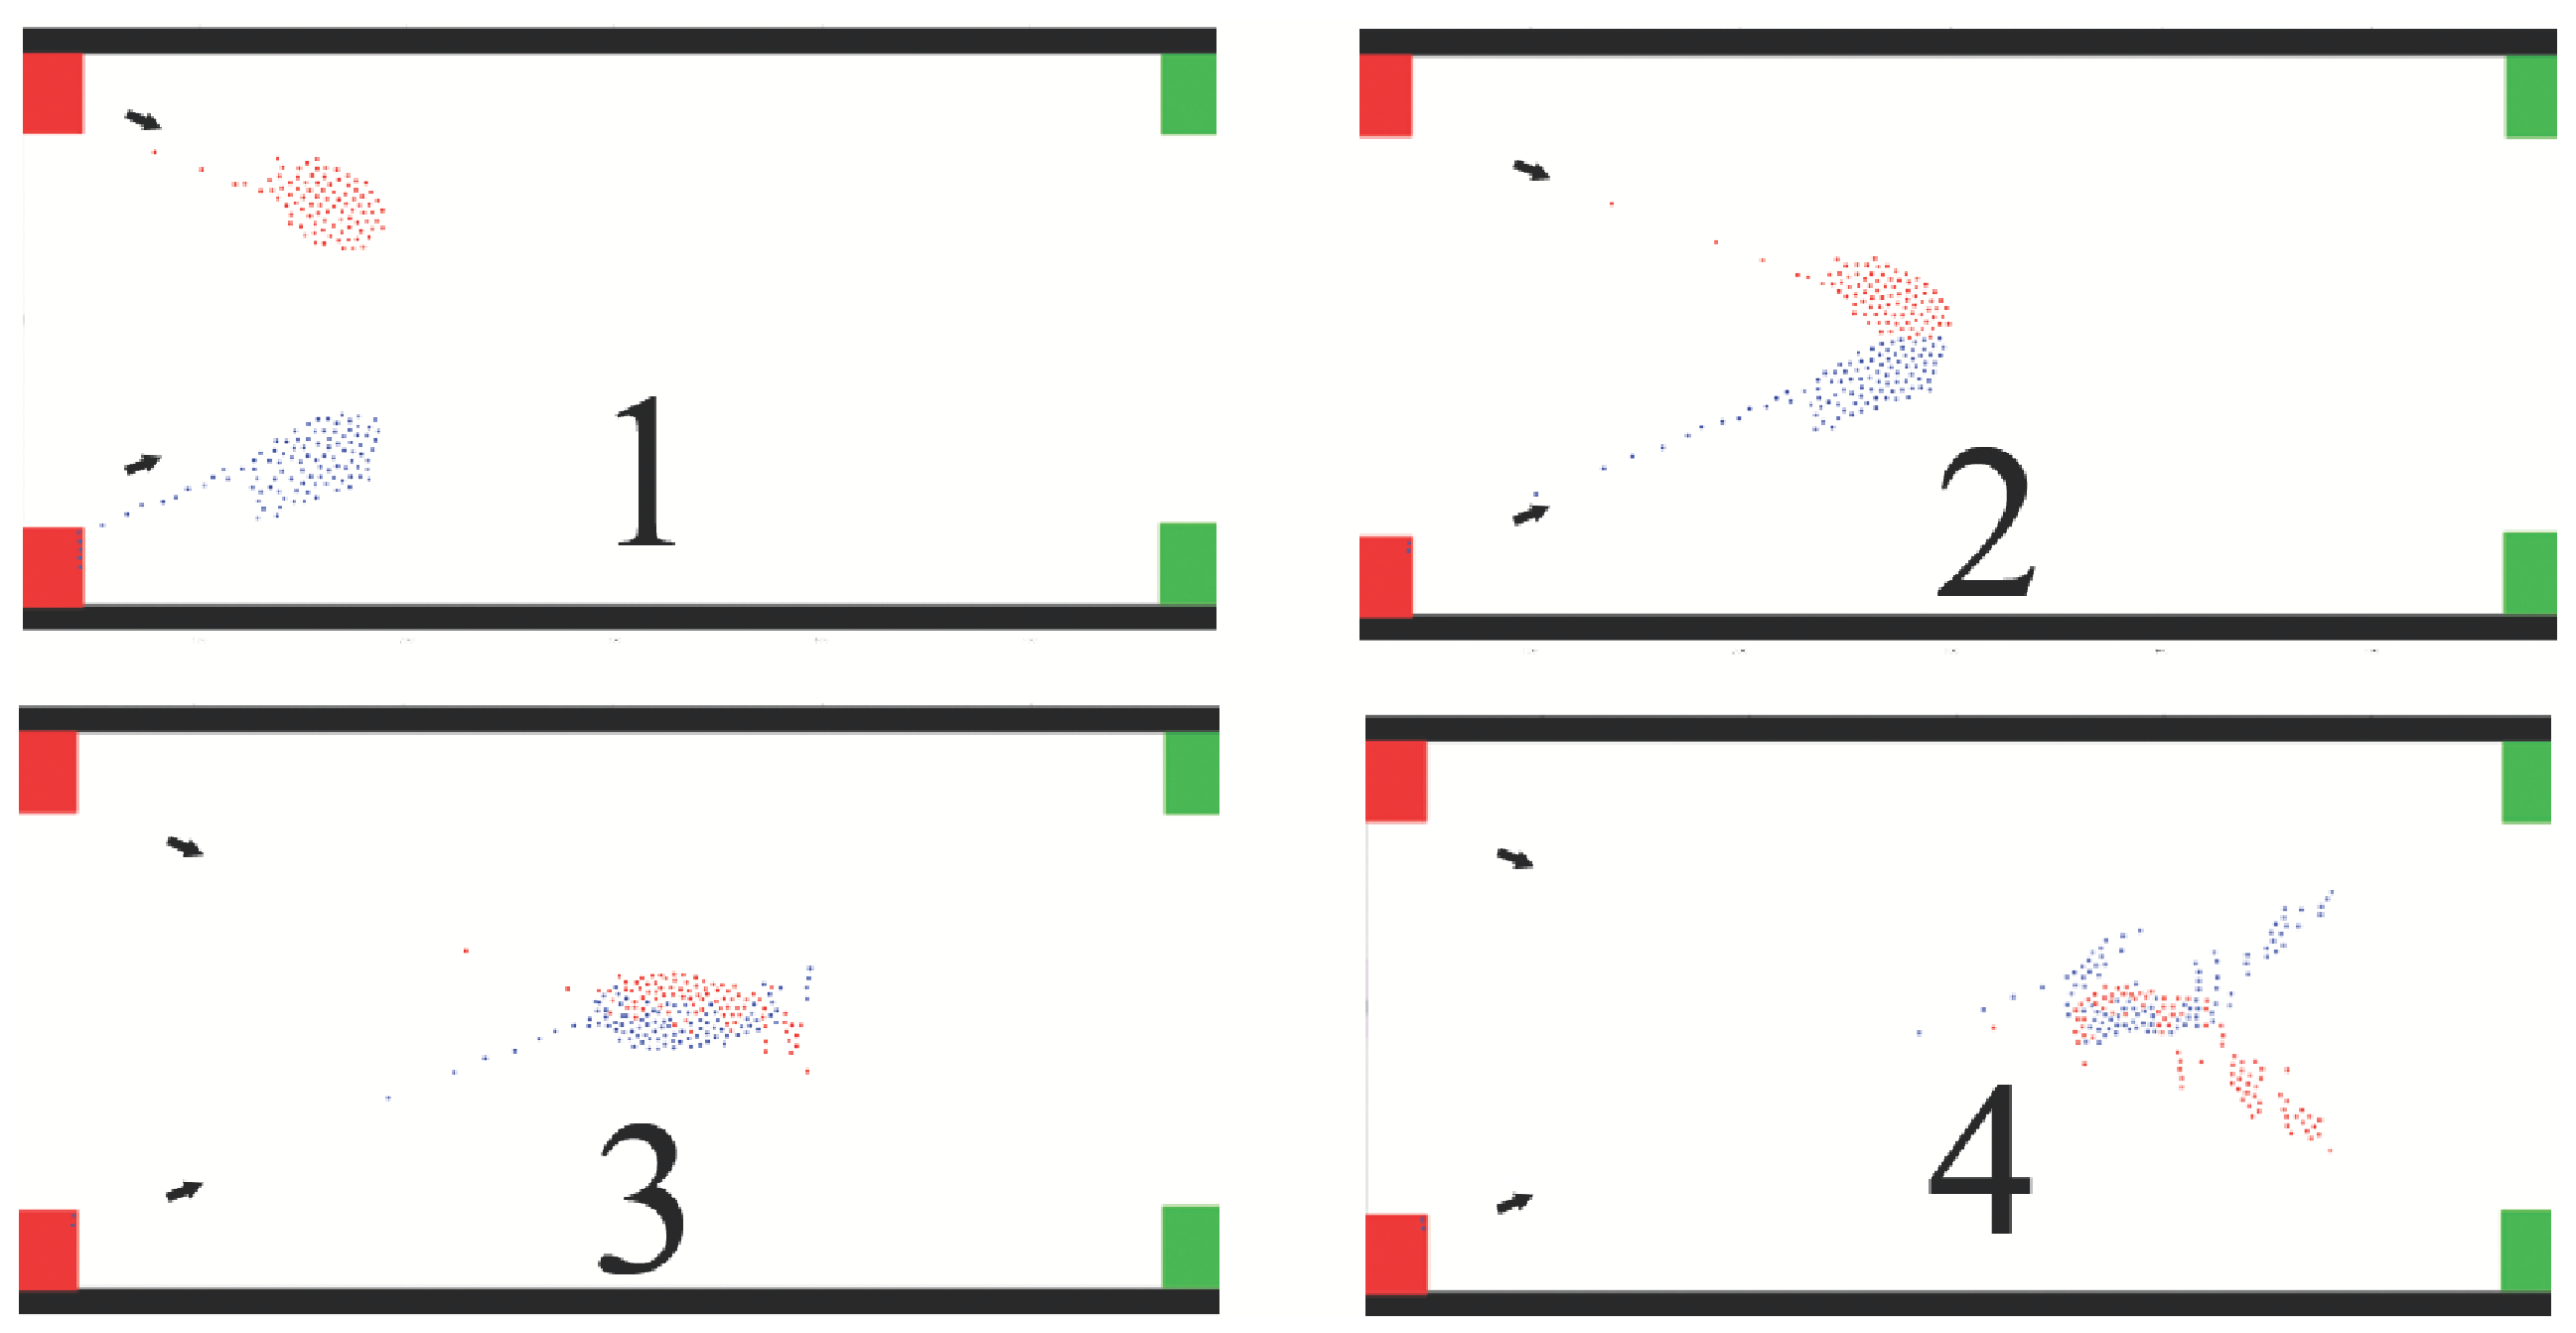
\includegraphics[bb=0bp 0bp 1311bp 661bp,width=1.05\columnwidth]{imgs/noque}

\caption{primitive simulation without queues }
\end{figure}


\noindent 
\begin{figure}
\noindent 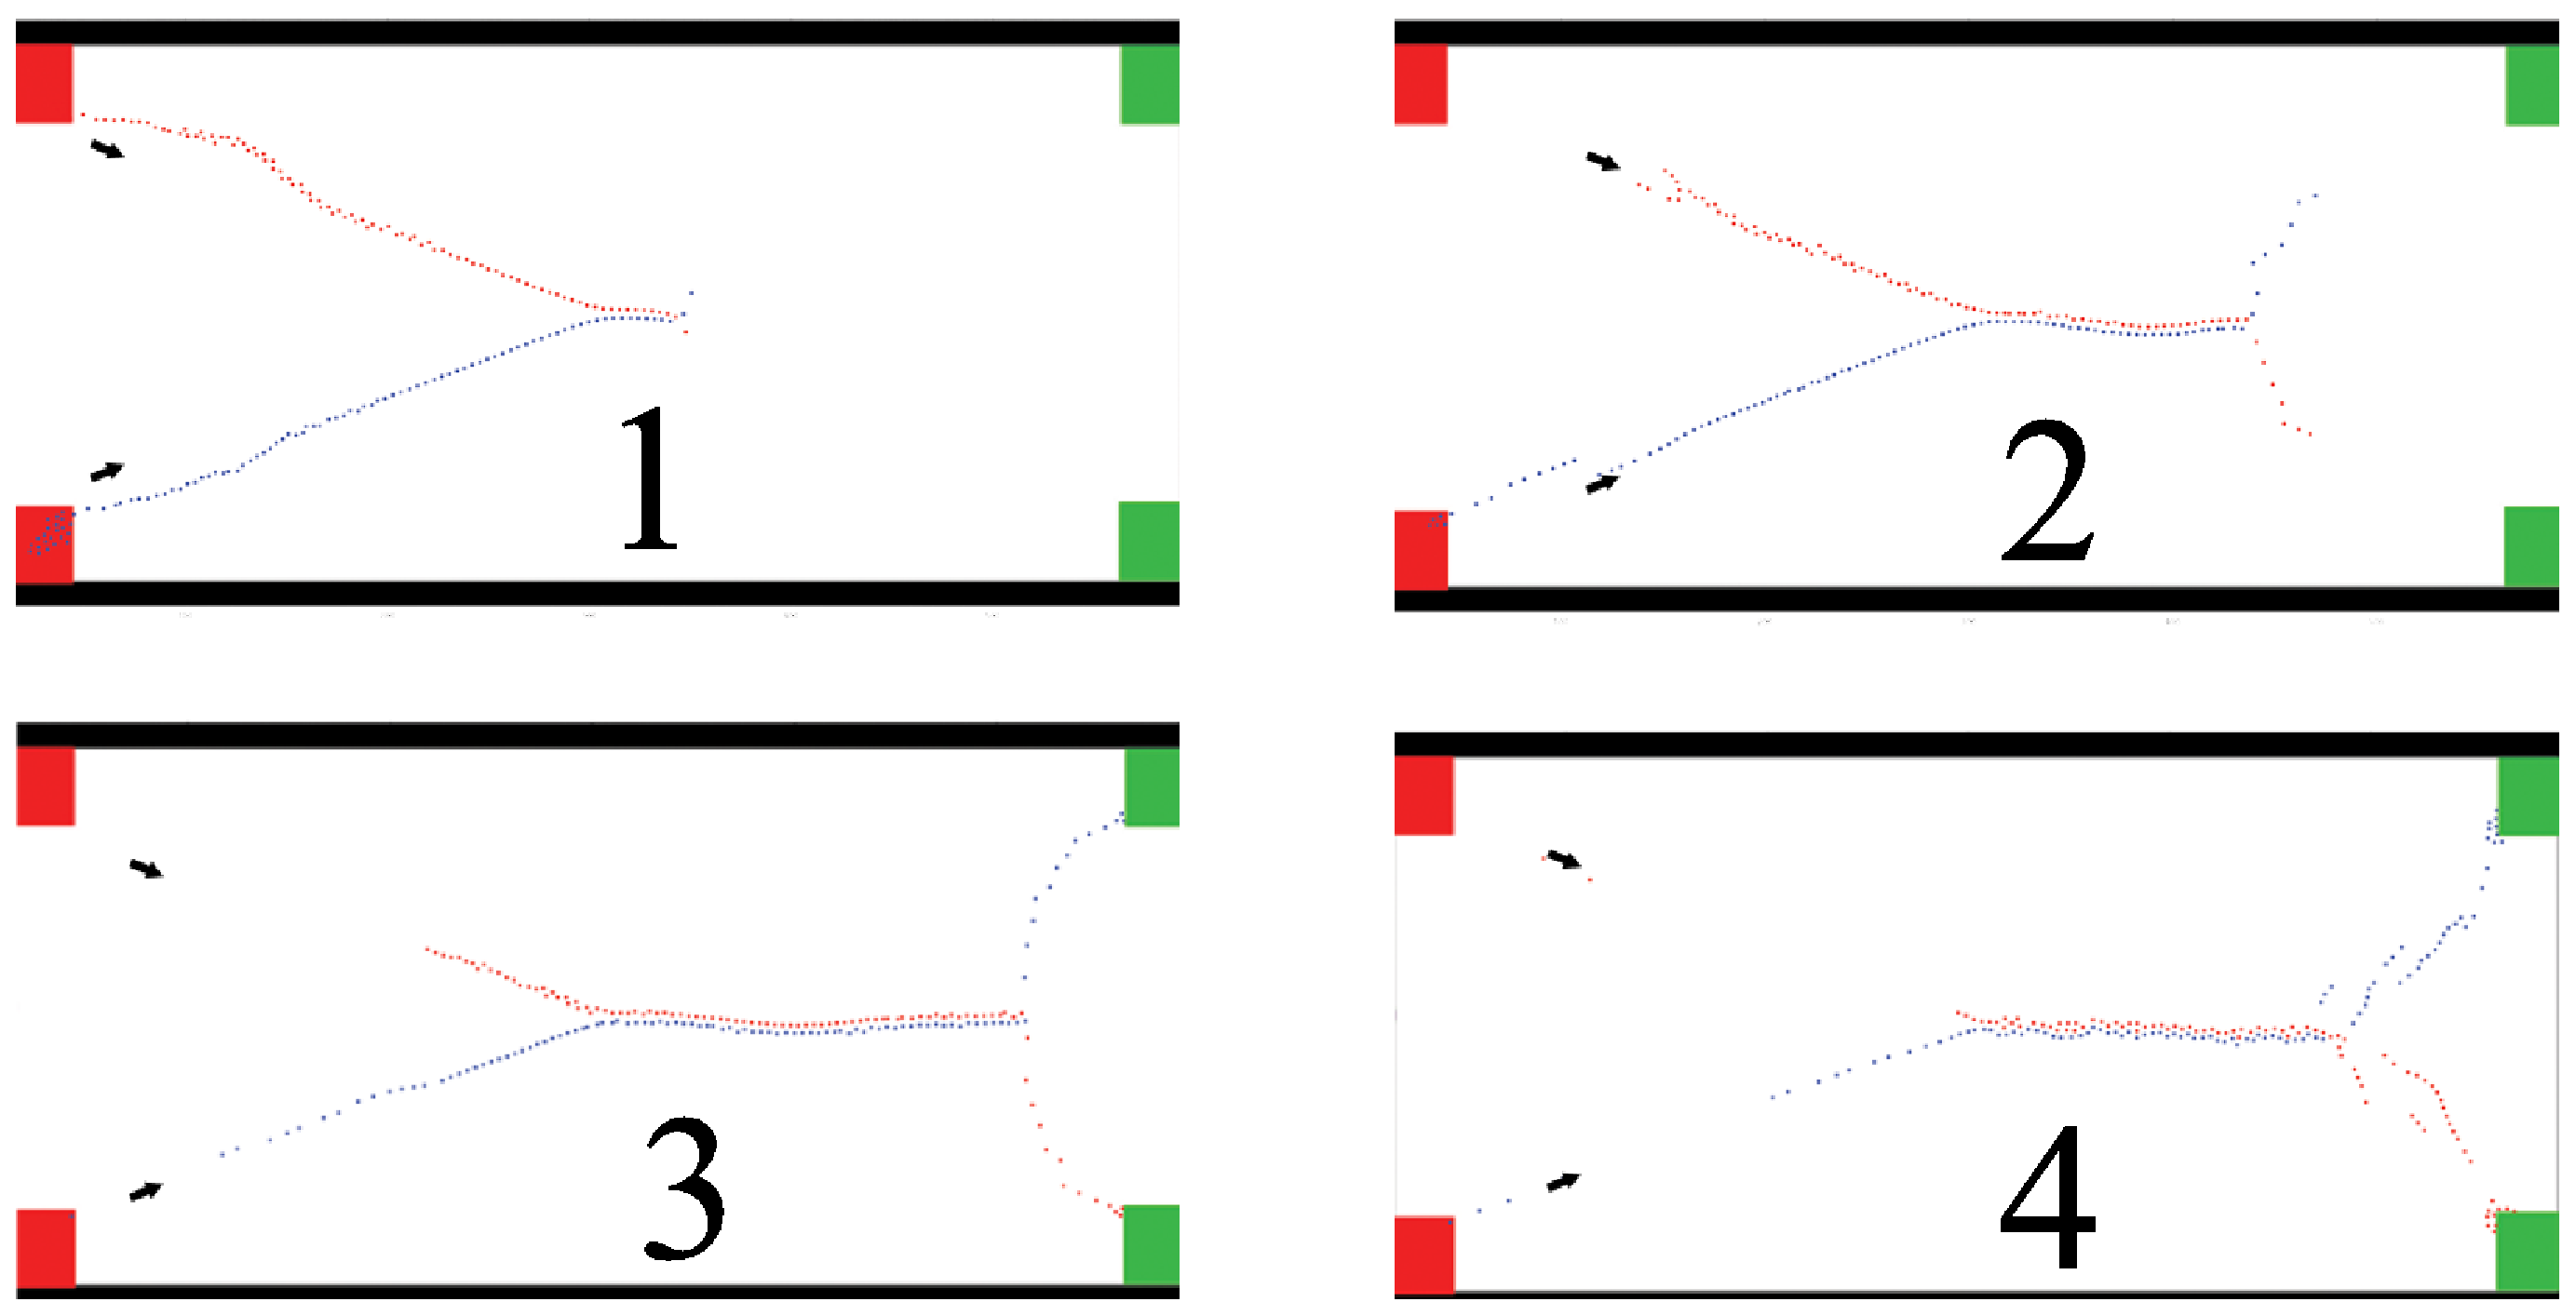
\includegraphics[width=1\columnwidth]{imgs/que}

\caption{primitive simulation with queues}
\end{figure}


\pagebreak{}

\selectlanguage{british}%

\subsection{Primitive Simulation with and without real-time fast marching algorithm}

In Figure 5. the difference between agents using the real time fast
marching algorithm are demonstrated. The differences are very apperant.
Without real time FM agents are realtively closely packe. On the other
hand, simulations using FM show agents more spread out taking the
mass of the crowd into account.

\begin{figure}
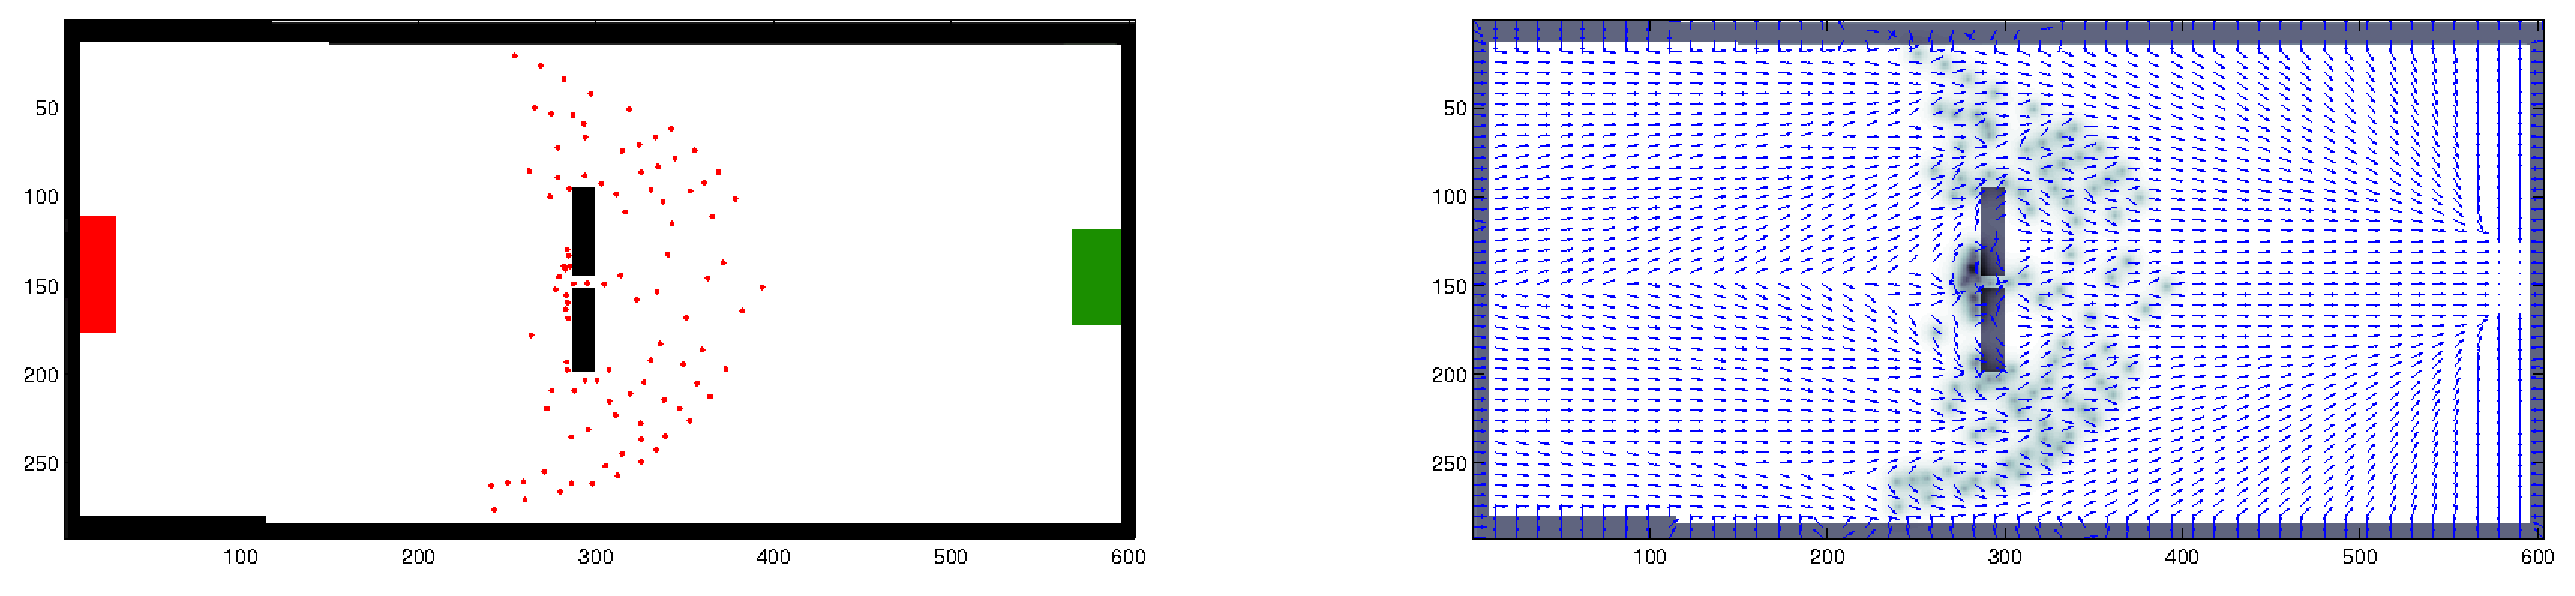
\includegraphics[width=1\textwidth]{simulation/fastmarchdemo/fm}

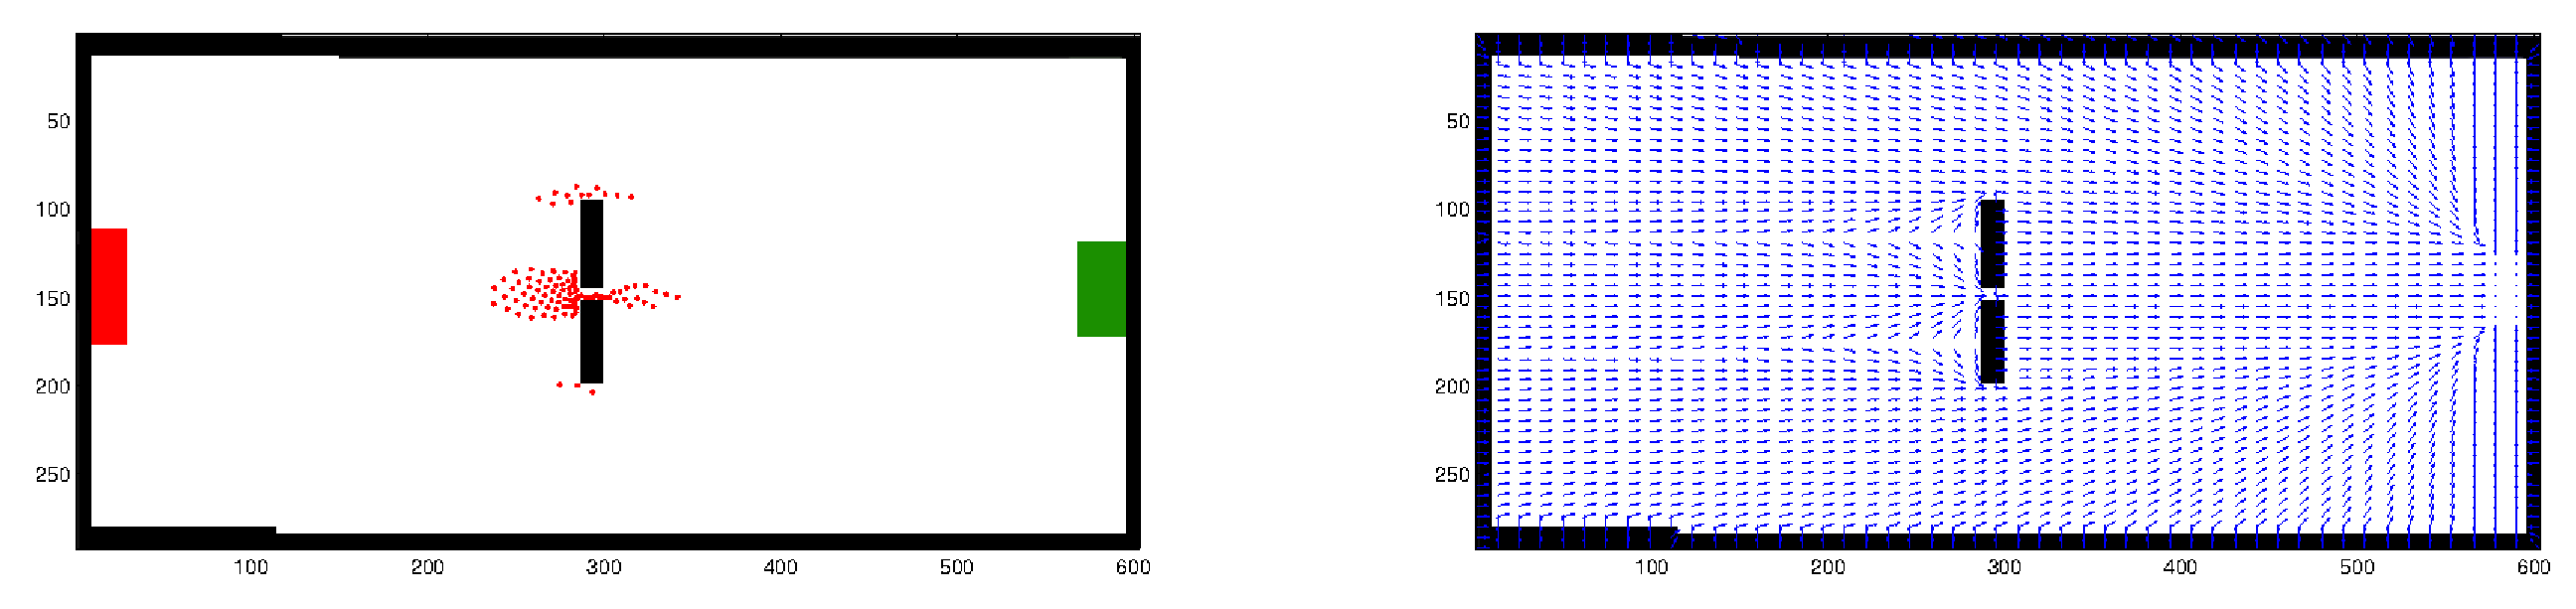
\includegraphics[width=1\columnwidth]{simulation/fastmarchdemo/nofm}\caption{Top is with Fast marching algorithm, bottom image without it.}
\end{figure}


\selectlanguage{english}%

\subsection{Parameterization for the Mensa}

To simulate hungry people rushing through the Mensa, a map based on
\emph{rauminfo.ethz.ch}%
\footnote{http://www.rauminfo.ethz.ch/Rauminfo/grundrissplan.gif?region=Z\&areal=Z\&gebaeude=MM\&geschoss=B%
} was constructed. The distribution of the agents to the different
{}``menus'' was done by rough estimation. It was estimate that about
10\% of mensa-goers decide to buy the \emph{bio-men�}. 
\begin{figure}
\includegraphics[height=5cm]{\lyxdot \lyxdot /src/maps/grundrissplan}\qquad{}\includegraphics[height=5cm]{\lyxdot \lyxdot /src/maps/grundrissplan3}\qquad{}\includegraphics[height=5cm]{\lyxdot \lyxdot /src/maps/grundrissplan4}

\caption{Map evolution process}
\end{figure}


While experimenting with different parameters, the walls had to be
thickened several times. Otherwise, agents were pushed through alls
due to the high forces.

The following plots are based upon 4000 to 5000 steps. Due to the
slow simulation (5000 steps take about 15 minutes), the {}``parameter-sweeping''
was done manually and very time consuming. Two exemplary problems
we ran into:


\paragraph*{Literally pitfalls}

\begin{figure}
\begin{centering}
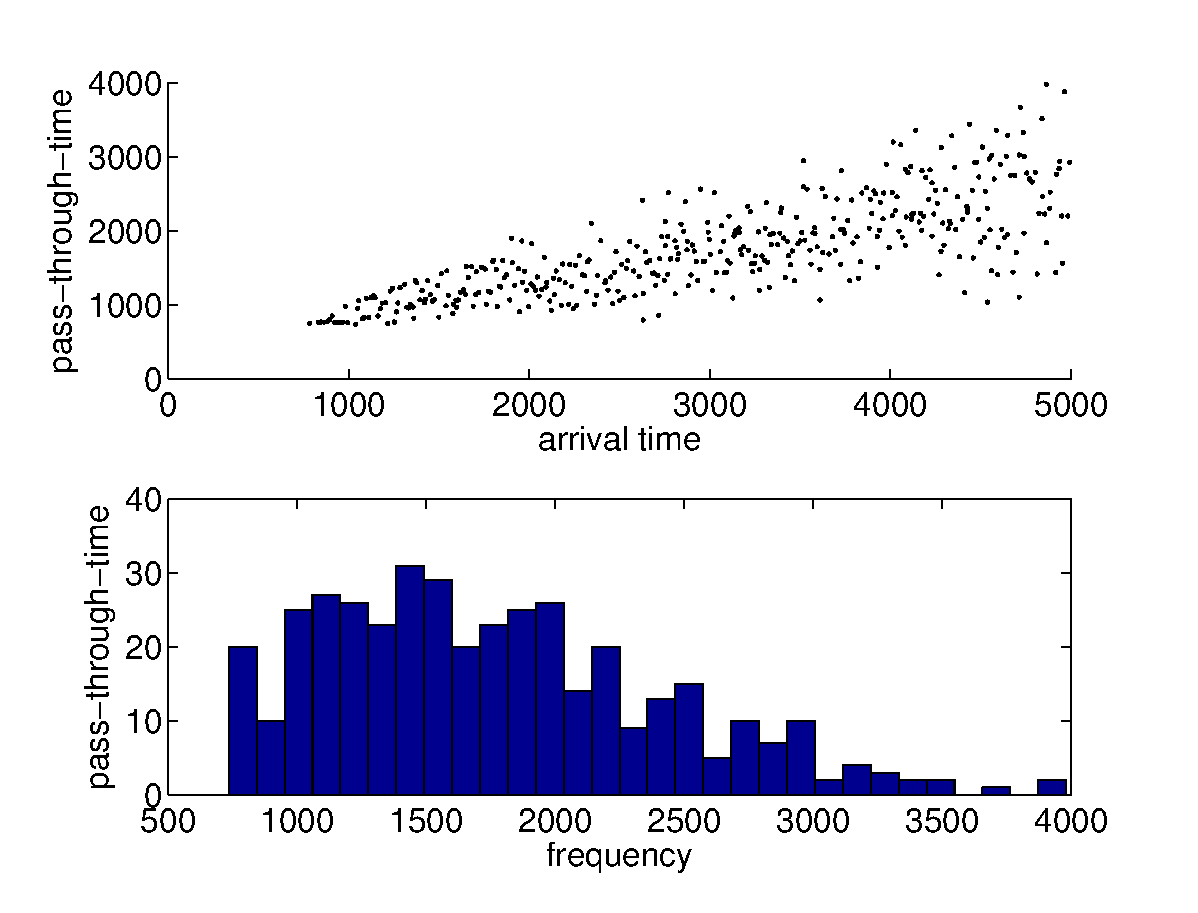
\includegraphics[width=8cm]{imgs/remote-worker-plots/fetchtime1}
\par\end{centering}

\caption{\label{fig:No-steady-state}No steady-state}
\end{figure}


With too few or slow checkouts, too many agents were trapped and no
{}``continuos flow of agents'' could be achieved. This can be verified
in figure \ref{fig:No-steady-state} which shows (in the upper part)
the agents' passing-through-time compared to their arrival time: No
upper limit seems to emerge. 


\paragraph*{High inrush}

After adapting some parameters (mostly \noun{meter}), the map needed
some tweaking to avoid unrealistically high inflow of agents (figure
\ref{fig:Tweaking-the-inflow}) which ultimately floods the mensa
with people.

\begin{figure}[H]
\begin{centering}
\includegraphics[height=7cm]{imgs/density_ungebremst}\qquad{}\includegraphics[height=7cm]{imgs/gebremst}
\par\end{centering}

\caption{\label{fig:Tweaking-the-inflow}Tweaking the inflow}
\end{figure}



\subsection{Comparing heuristics}

With the found parameters (see Appendix on p.~\pageref{sub:Parameters}),
a benchmark of our heuristic was done. The first run included just
the \textbf{bare social-force model}, the second run used our \textbf{{}``simple
queueing''} and the third featured \textbf{real-time fast marching
}as well as our \textbf{queueing} extension (Shown from left to right
in the following three plots).


\paragraph{Pass-through-time}

In figure \ref{fig:arrival}, an {}``upper limit'' for the pass-through-time
shows up in all three runs: thus, no agents got stuck for very long
periods of time. The different heuristics however do not seem to impact
the passing-through-time.

\begin{figure}[H]
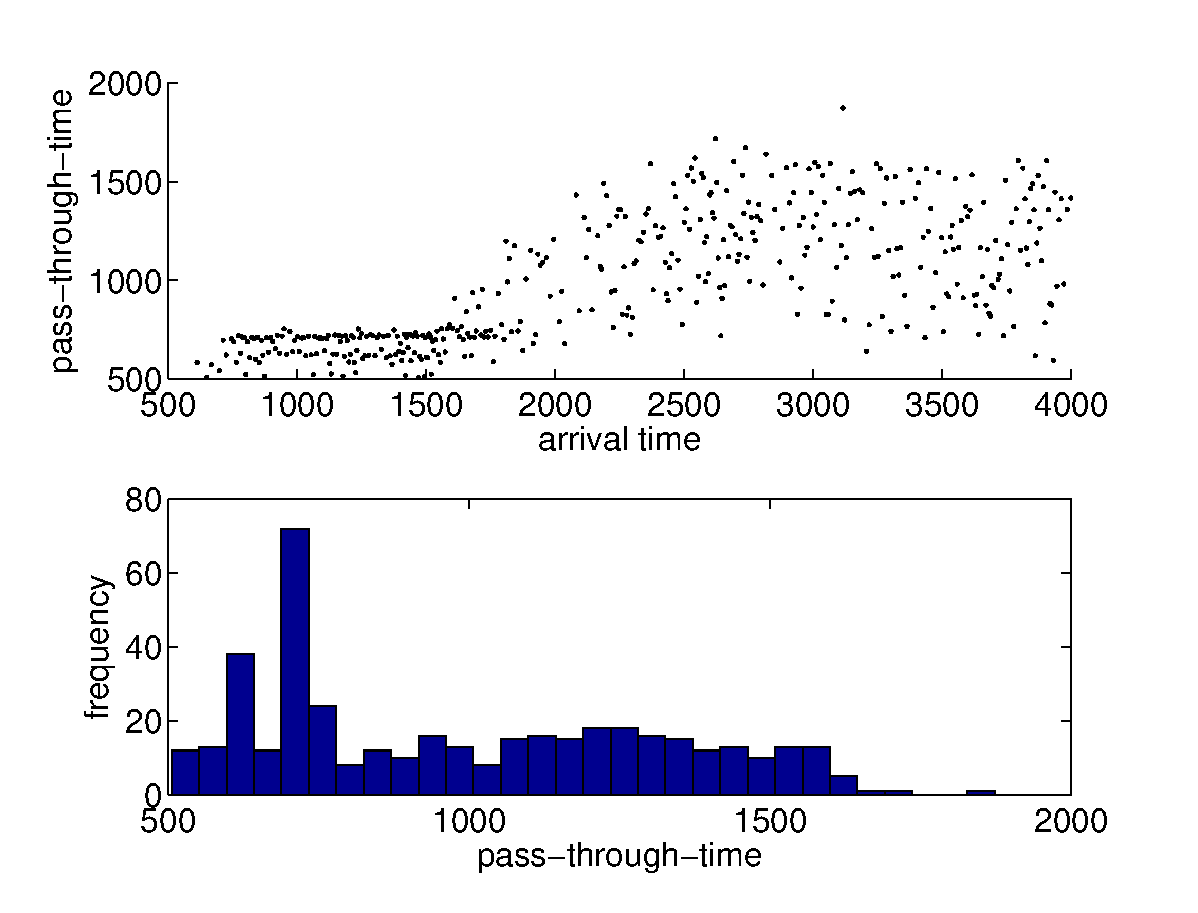
\includegraphics[width=0.32\textwidth]{simulation/nofm_noque/arrival}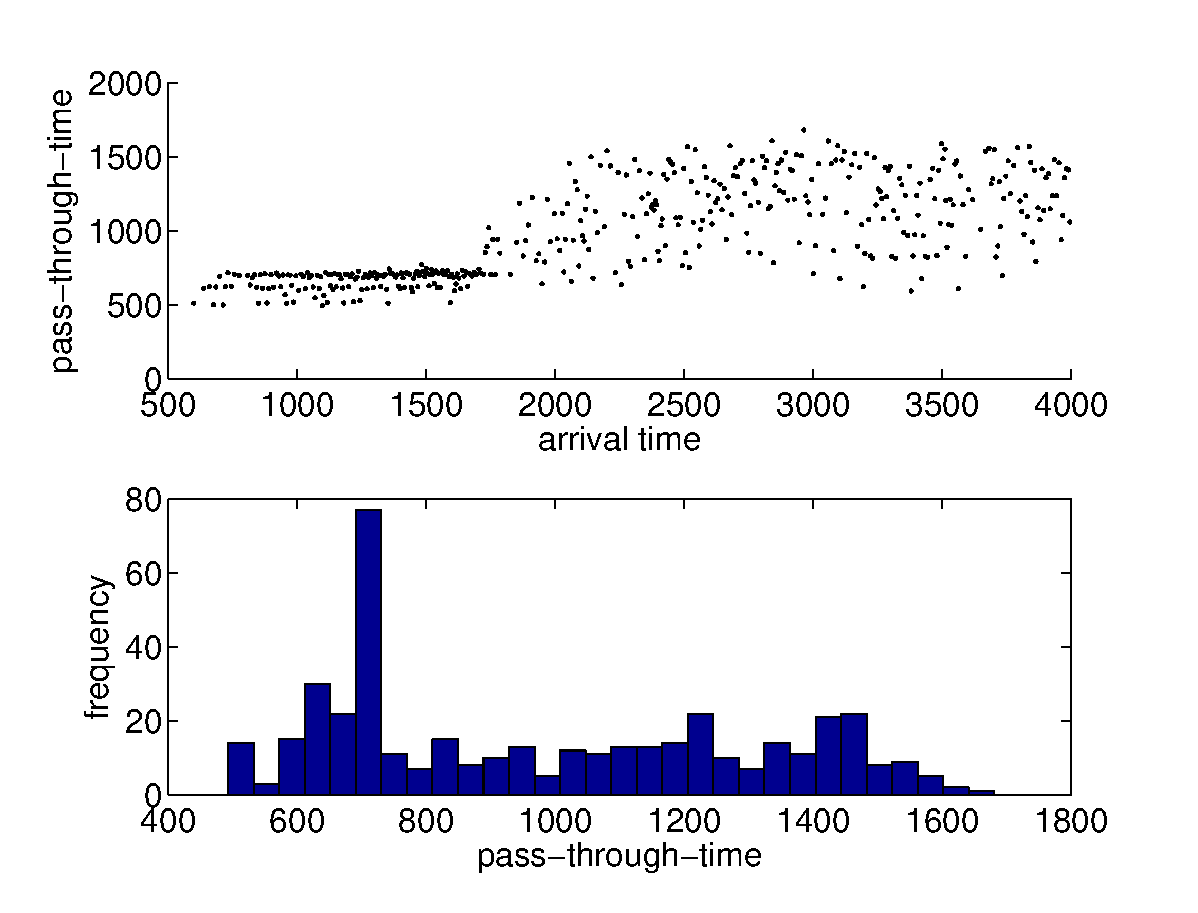
\includegraphics[width=0.32\columnwidth]{simulation/nofm_que/arrival}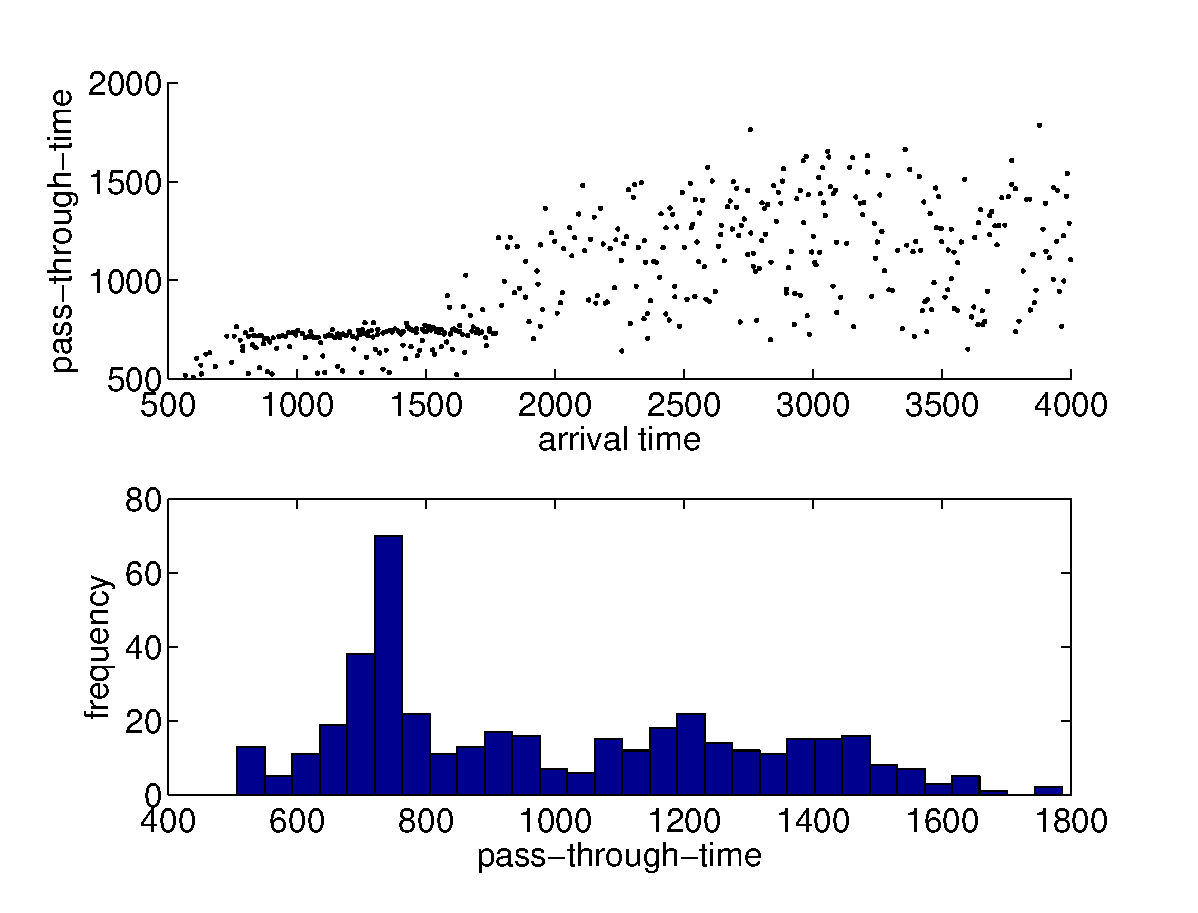
\includegraphics[width=0.32\columnwidth]{simulation/fm_que/arrival}

\caption{\label{fig:arrival}Pass-through-time}
\end{figure}



\paragraph{}


\paragraph{Space usage}

In the third comparison, the effort made finally pays of: By adding
queuing heuristics (left vs. center image), it can be seen how the
crowd just in front of the upper left service sparses. It can be concluded
that queue aware agents rush less.

\selectlanguage{british}%
By recalculating the fast-marching-paths (center vs. right image),
agents realise the crowd in their way and take longer, but quicker
ways to other checkouts.

\selectlanguage{english}%
\begin{figure}[H]
\includegraphics[height=5.5cm]{simulation/nofm_noque/dens} \includegraphics[height=5.5cm]{simulation/nofm_que/dens}
\includegraphics[height=5.5cm]{simulation/fm_que/dens}

\caption{Comparing space usage}
\end{figure}
\foreignlanguage{british}{In the following screencaptures -- and way
better in the videos -- we can see how the agents on their way to
the checkout move more flexible with the real-time-fast-marching.}

\selectlanguage{british}%
\begin{figure}[H]
\includegraphics[width=0.3\textwidth]{simulation/fm_que/snapshots/10s}\ \includegraphics[width=0.3\textwidth]{simulation/nofm_noque/snapshots/10s}\ \includegraphics[width=0.3\textwidth]{simulation/nofm_que/snapshots/10s}

\caption{Simulation after 300 Frames, from left to right. 1. with queues, with
fast marching, 2. without queues, with fast marching 3. with queues,
without fast marching }
\end{figure}


\noindent 
\begin{figure}[H]
\includegraphics[width=0.3\textwidth]{simulation/fm_que/snapshots/1m}\ \includegraphics[width=0.3\textwidth]{simulation/nofm_noque/snapshots/1m}\ \includegraphics[width=0.3\textwidth]{simulation/nofm_que/snapshots/1m}

\caption{Simulation after 1800 Frames from left to right. 1. with queues, with
fast marching, 2. without queues, with fast marching 3. with queues,
without fast marching }
\end{figure}


\noindent 
\begin{figure}[H]
\includegraphics[width=0.3\textwidth]{simulation/fm_que/snapshots/2m}\ \includegraphics[width=0.3\textwidth]{simulation/nofm_noque/snapshots/2m}\ \includegraphics[width=0.3\textwidth]{simulation/nofm_que/snapshots/2m}

\caption{Simulation after 3600 Frames, from left to right. 1. with queues,
with fast marching, 2. without queues, with fast marching 3. with
queues, without fast marching }
\end{figure}


Figures 11- 13 show screencaptures of the videos which were made whilst
collecting the data presented in Section 5.3. In these screencaptures
-- which are available as videos on github -- it can be see how the
agents on their way to the checkout move more flexible with the real-time-fast-marching.

\selectlanguage{english}%

\section{Summary and Outlook}

Building mainly on the concepts published by the {}``Social Force
Model of Pedestrian dynamics'' (1995) and {}``Self-organized Pedestrian
Crowd Dynamics'' (2005) which were both published by Dirk Helbing
et al. an algorithm to simulate crowd behaviour was implemented. The
task was to fabricate a concrete model derived from these general
models. The models were to some extent modified and extended to realistically
simulate crowd behaviour in the ETHZ Polymensa. Summarized, the added
extensions were queue heuristics as well as crowd destination dynamics
(first the different meals, then the cash register) which are described
in detail in sections 4 and 5. 

The simulations showed characteristics which group members have observed
to exist (see Section 5.2), but the reproduction of a realistic queue
turned out to be much more demanding than expected. Further improvements,
such as agents who estimate their neighbours' speed and include this
in their path planning, urge to be implemented.

From the current results it is not yet possible to draw a conclusion
concerning the degree of realism of the simulation. In order to this,
empirical data would have to be collected. This information could
then be compared to simulated data. In a further step empirical data
could be collected from various mensas which could also be simulated.
If these prove to be realistic with only little modification of the
model, then the simulation could be used as an aid in the architectural
design of mensas. It is only possible through the extensive collection
of empirical data to draw conclusions about empirical reality from
computer simulated reality which was outside the scope of this report.

\selectlanguage{british}%

\subsection{References}
\begin{itemize}
\item \emph{Social Force Model for Pedestrian dynamics (1995) -- Dirk Helbing
et al. }\\
Describes model we are considering to build on (Social Force Model)
\item \emph{Self-organized Pedestrian Crowd Dynamics (2005) -- Helbing et
al. }\\
Uses model we are considering to build on (Social Force Model)
\item \emph{Pedestrian Dynamics Airplane Evacuation Simulation -- Author(s):
P. Heer, L. B�hler }\\
Model we are considering to build on (Social Force Model)
\item \emph{Response to intrusion into waiting lines. (2010) By Milgram,
Stanley et al.}%
\footnote{http://psycnet.apa.org/index.cfm?fa=buy.optionToBuy\&id=1987-04011-001 %
} \\
A possible extension to queue modeling. This extension would include
intruders which are more aggressive and attempt to intrude into waiting
lines.
\item \emph{Approach to Collective Phenomena in Pedestrian Dynamics (2002)
Andreas Schadschneider et al. }\\
In case we attempt to use Cellular Automata this paper would be useful. 
\item \emph{Writing Fast MATLAB Code (2004) -- Pascal Getreuer}
\end{itemize}

\section{Appendix}


\subsection{Source Code}

All the source code is stored in the directory 'src/'


\subsubsection{Agents Forces \texttt{| agents\_force.m}}

\lstinputlisting{../src/agents_force.m} 

\selectlanguage{english}%

\subsubsection{Count Passes \foreignlanguage{british}{\texttt{| count\_passes.m}}}

\lstinputlisting{../src/count_passes.m}


\subsubsection{Init Agents \foreignlanguage{british}{\texttt{| init\_agents.m}}}

\lstinputlisting{../src/init_agents.m}

\selectlanguage{british}%

\subsubsection{Parameters\label{sub:Parameters}}

\lstinputlisting{../src/parameters.m}


\subsubsection{Plot Stat \texttt{| plot\_stat.m}}

\lstinputlisting{../src/plot_stat.m}


\subsubsection{Potential Force \texttt{| potential\_force.m}}

\lstinputlisting{../src/potential_force.m}


\subsubsection{Refresh Fields \texttt{| refresh\_fields.m}}

\lstinputlisting{../src/refresh_fields.m}


\subsubsection{Remote Worker \texttt{| remote\_worker.m}}

\lstinputlisting{../src/remote_worker.m}


\subsubsection{Reset Simulation \texttt{| reset\_sim.m}}

\selectlanguage{english}%
\lstinputlisting{../src/reset_sim.m}

\selectlanguage{british}%

\subsubsection{Separate Areas \texttt{| seperateAreas.m}}

\lstinputlisting{../src/seperateAreas.m}


\subsubsection{Simulate \texttt{| simulate\_v1.m}}

\lstinputlisting{../src/simulate_v1.m}


\subsubsection{Test Agents Force \texttt{| test\_agents\_force.m}}

\lstinputlisting{../src/test_agents_force.m}


\subsubsection{Test Load Map \texttt{| test\_load\_map.m}}

\lstinputlisting{../src/test_load_map.m}
\end{document}
